\section{So you want to know how the brain works?}
\label{sec:1_brain}

How a convoluted network of synapses can enable an animal to think and exhibit complex behavior has been a motivating question of neuroscience since the discovery of neurons in the late 19\textsuperscript{th} century \cite{ramon1899textura, finger2001origins}. Neuronal circuit diagrams, maps delineating the connections between synapses, have shown to be useful tools for better understanding cognitive function and neural architecture \cite{helmstaedter20083d, kasthuri2015saturated}. Although several full brain circuit diagrams have been completed (C. elegans \cite{white1986structure}, fruit fly larva \cite{ohyama2015multilevel}, tunicate tadpole larva \cite{ryan2016cns}, zebrafish larva \cite{hildebrand2017whole}, and adult fruit fly \cite{zheng2018complete}), such ``connectomes" are a herculean task given that the resolution required to discern synapses is on the nanometer scale, while the organ as a whole spans millimeters or larger, depending on the organism \cite{lichtman2008ome, bock2011network, kornfeld2018progress}. Electron microscopy (EM), an imaging technique able to reach magnification scales several orders of magnitude higher than light microscopy by illuminating a specimen with a beam of accelerated electrons, is currently the only imaging method capable of resolving such fine features across such vast spatial extents \cite{helmstaedter20083d, zheng2018complete}. The drawback for high-magnification imaging over organ-scale dimensions is, however, the inherently limited throughput, leading to hours or days of acquisition time for a single two-dimensional cross section. Extending acquisitions of biological material to the third dimension has long remained a challenge for EM.

While the brain is perhaps the most prominent, it is certainly not the only example in biology where multi-scale microscopy can assist in mapping connectivity relations crucial to functional performance. Molecular-scale processes taking place within cells or organelles are highly regulated in health, and defects or deviations at the smallest scales can lead to dysfunction or disease at the organ or organism level. Simply put, the big things are made out of lots of little things, and to figure out how the big thing works, you have to look at all the little things. EM is the only technique that can see the littlest things and that might do this over the full size of the big things.


% --- VEM ---
\section{Volume electron microscopy}
\label{sec:1_vEM}

There are a variety of techniques for three-dimensional imaging of biological specimen via electron microscopy (EM) \cite{peddie2014exploring}. Modern volume EM techniques can be divided into two broader methods: array tomography approaches, in which ultrathin serial sections are cut from a block of tissue prior to EM (e.g. serial section scanning EM or transmission EM), and blockface approaches, in which the tissue block is sectioned as it is imaged (e.g. serial blockface or focused ion beam SEM). While both of these approaches have their respective advantages and disadvantages \cite{briggman2012volume, peddie2014exploring}, an important distinction is that array tomography allows for re-evaluation of sections whereas the specimen is irrevocably lost in blockface approaches \cite{schifferer2021niwaki}.

Despite the success these techniques have had in generating high-quality three-dimensional reconstructions, significant challenges remain. At present, one of the most stringent constraints facing high-resolution (<\,\SI{10}{\nano\meter}) volume EM is throughput. To scan an entire mouse cortical column, for example, a $400 \times 400 \times \SI{1000}{\micro\meter^3}$ volume, at \SI{4}{\nano\meter\per\pixel} with \SI{30}{\nano\meter} section thickness (the resolution necessary to reliably discern synapses \cite{harris1989dendritic, meinertzhagen1991synaptic}), \textcite{briggman2012volume} estimated that it would require ${\sim}$\SI{500}{days} of uninterrupted imaging with a single beam. For this reason, it is advantageous to locate regions of interest prior to large-scale EM in order to minimize the imaging volume.

One approach, taken by \textcite{hildebrand2017whole} for whole-brain serial section SEM reconstruction of a larval zebrafish, was to utilize multiple rounds of targeted EM at successively higher levels of magnification. Similar approaches have been taken in other large-scale neural reconstruction endeavors such as partial brain imaging of a mouse visual cortex \cite{bock2011network} and full brain imaging of an adult fruit fly \cite{zheng2018complete} where certain synapses were re-imaged at higher resolution. Although these multiscale approaches have been implemented with great success, the need for intermediate analysis of the EM dataset hinders throughput. The selection of sub-regions of interest for subsequent imaging rounds is driven by localization of the biological material of interest, which can only be done after manual or machine-learning-assisted analysis of the preceding EM dataset. While machine-learning techniques have made tremendous progress in reducing human involvement, interpretation and annotation of EM datasets remain a tedious and error-prone practice. These methods are therefore not yet appropriate for selecting sub-regions at higher magnification scales, meaning selection cannot be done either automatically or in real time.


% --- CLEM ---
\section{Correlative light and electron microscopy}
\label{sec:1_CLEM}

In addition to low throughput, EM has the additional limitation that it does not contain the protein- and molecular-specific information available from fluorescence microscopy (FM)---unless the proteins are known to be specifically linked to a structural component. This information is not only crucial for understanding biological function but can also be used to guide to regions of interest (ROI) based on molecular expression. Thus, while EM is successful at providing ultrastructural information, it is not always useful for localizing ROIs. Functional fluorescence microscopy has been employed to identify the biological material of interest, particularly in blockface approaches \cite{karreman2016fast}. However, workflows to retrieve selected regions from the specimen and trim the block to the appropriate size can be both complicated and time-consuming or involve further rounds of multimodal inspection, e.g. with X-ray tomography \cite{karreman2016intravital}. Linking between the structural information conveyed by EM and the dynamic, functional data obtained with live-cell FM can furthermore be challenging when EM is performed following FM and the intermediate sample preparation \cite{de2015correlated}.

As the advantages afforded by merging targeted biological information with ultrastructural detail often outweigh the challenges, methods have been developed for combining FM and EM in correlative light and electron microscopy (CLEM). In the past decades, CLEM has evolved from being used by only a few pioneering, specialist labs to a collection of techniques and workflows practiced by a broad group of researchers in structural biology \cite{de2015correlated, ando20182018}. In most cases, CLEM involves a distinct set of sequentially used specimen preparation and labeling techniques, followed by diverse types of light and electron microscopy techniques, with specific workflows for sample transfer and relocation of regions of interest. A key advantage of sequential CLEM is the wide diversity of available microscopes: in principle, any type of microscope can be added to the workflow, provided requirements on sample preparation and handling can be met. Procedures to combine different light and electron microscopes can, however, be tedious, involving extensive manual labor, transfers, and cumbersome ROI retrieval.


% --- Integrated microscopy ---
\section{Integrated microscopy}
\label{sec:1_integrated}

Microscopes that integrate a light and an electron microscope in one have been developed as early as the 1980s and a wide variety of integrated microscopes with different modalities has been reported in literature in recent years \cite{zonnevylle2013integration, timmermans2015contributed}. Several of these have now also become commercially available. For a specific CLEM experiment, the choice between an experimental workflow with standalone microscopes or with an integrated microscope depends on a variety of factors: the precise goal and requirements of the experiment, amenable sample preparation protocols, and local availability of microscopes, probes, and expertise. If only a single or very few samples have to be carried through the CLEM workflow, adopting sample preparation protocols towards integrated inspection may not be worth the effort. On the other hand, integrated microscopes offer advantages in terms of throughput, avoiding sample contamination, achievable precision of ROI retrieval, and ease and accuracy of image correlation.


% --- Integrated array tomography
\section{Integrated correlative array tomography}
\label{sec:1_iCAT}

The advantages offered by integrated microscopy extend to volume imaging. In conventional array tomography, a tissue specimen is chemically fixated, embedded in resin, and cut into a series of ultrathin sections which are collected as ribbons on a solid substrate or on flexible, sticky Kapton tape. The sections are then immunostained for imaging in a widefield or confocal fluorescence microscope, possibly in several rounds to target multiple molecules. Next, the sections are washed and reprocessed for EM with e.g. osmium tetroxide or uranyl acetate and transferred to a scanning or transmission electron microscope \cite{micheva2007array, wacker2013array}. Integrated array tomography seeks to advance this workflow by combining FM and EM acquisition with the high alignment accuracy and automation afforded by an integrated light and electron microscope. While the need for intermediate sample preparation is removed, it does, however, impose stricter constraints on the amount of heavy metal staining that can be used for EM to avoid quenching fluorophores \cite{kuipers2015scanning, peddie2017correlative}. To circumvent the loss of signal without increasing the dwell time, a negative bias potential can be used to enhance the collection of backscattered electrons (Chapter \ref{chap:2}).

% Figure 1.1 (iCAT)
% -----------------
\begin{figure}[!tb]
    \centering
    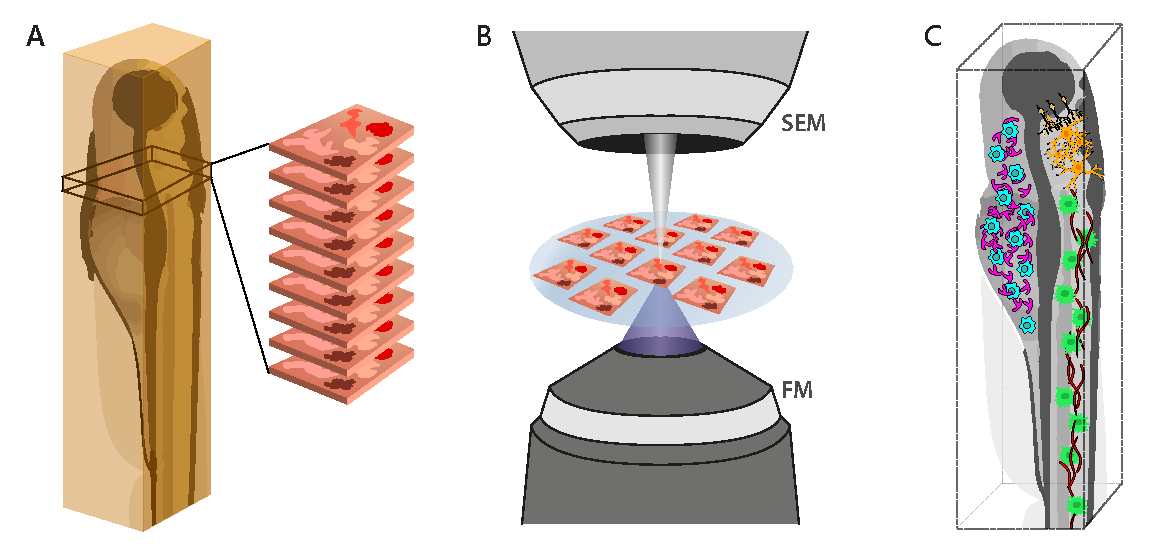
\includegraphics[width=\linewidth]{chapter-1/figures/fig1_iCAT_v2.pdf}
    \caption{Conceptual overview of the integrated array tomography workflow.
    (A) Serial sections are cut from a resin-embedded specimen; a larval zebrafish is illustrated here as an example.% The sections are then placed onto an ITO-coated glass slide, and prepared for simultaneous CLEM.
    (B) The sections are placed onto an ITO-coated glass slide which is mounted onto the translation stage of the integrated microscope. A series of registered EM-FM image pairs are acquired according to a semi-automated imaging pipeline.
    (C) The EM images are computationally aligned in 3D, revealing the structure of the zebrafish. The fluorescence data, comprising the targeted organelles, proteins, or biomolecules, is then overlaid onto the EM, resulting in a volume CLEM reconstruction of the zebrafish.
    Larval zebrafish illustration derived from original artwork by Lizzy Griffiths.}
    \label{fig:1.1_icat}
\end{figure}

The workflow for integrated correlative array tomography (iCAT; Fig. \ref{fig:1.1_icat}) begins by following a customized protocol for fixating, embedding, cutting, and immunolabeling a sample such that the fluorescence is maintained. Serial sections are then loaded into the integrated microscope and imaged sequentially, while an automated procedure for EM-FM registration \cite{haring2017automated} ensures consistent overlay accuracy. Custom-built alignment routines are then used to reconstruct the correlative datasets in three-dimensions. The acquisition and reconstruction procedures for integrated array tomography comprise the basis of Chapter \ref{chap:3}.

Future applications of CLEM will demand greater precision, further automation, and higher throughput, for which iCAT offers a number of potential advantages. Above all, iCAT enables large numbers of serial sections to be sequentially and automatically imaged to generate reconstructed volumes of overlaid FM and EM datasets with matching axial resolution. Moreover, specimen warping and shrinkage, which might otherwise occur in conventional array tomography methods, is prevented due to the absence of intermediate sample preparation. This ensures a precise overlay of biological molecules and structural context at high resolution in all three dimensions. Additionally, precisely overlaid fluorescence data has the potential to vastly improve classification of ultrastructural features in EM data. While modern machine-learning-based segmentation methods (e.g. ilastik \cite{sommer2011ilastik}, SuRVoS \cite{luengo2017survos}) are quite sophisticated, they nevertheless require some degree of manual annotation. Because high-accuracy overlaid correlative datasets contain, in a sense, the classification data that these methods seek to provide, such datasets could reduce the need for supervised learning while opening up new possibilities for machine learning applications such as artificial fluorescence predictions (Chapter \ref{chap:4}). 
